% !TEX root = saveliev_physics_general_course_2.tex
%!TEX TS-program = pdflatex
%!TEX encoding = UTF-8 Unicode


\chapter[STEADY ELECTRIC CURRENT]{STEADY ELECTRIC CURRENT}\label{chap:5}
\chaptermark{STEADY ELECTRIC CURRENT}

\section{Electric Current}\label{sec:5_1}

If a total charge other than zero is carried through an imaginary surface, an \textbf{electric current} (or simply a \textbf{current}) is said to flow through this surface. A current can flow in solids (metals, semiconductors), liquids (electrolytes), and in gases (the flow of a current through a gas is called a gas discharge).

For a current to flow, the given body (or given medium) must contain charged particles that can move within the limits of the entire body. Such particles are called \textbf{current carriers}. The latter may be electrons, or ions, or, finally, macroscopic particles carrying a surplus charge (for example, charged dust particles and droplets).

A current is produced if there is an electric field inside a body. The charge carriers participate in the molecular thermal motion and, consequently, travel with a certain velocity $\vec{v}$ even in the absence of a field. But in this case, an identical number of carriers of either sign pass on the average in both directions through an arbitrary area mentally drawn in the body, so that the current is zero. When a field is switched on, ordered motion with the velocity $\vec{u}$ is superposed onto the chaotic motion of the carriers with the velocity $\vec{v}$\footnote{Similarly, in a gas flow, ordered motion is superposed onto the chaotic thermal motion of the molecules.}. The velocity of the carriers will thus be $\vec{v}+\vec{u}$. Since the mean value of $\vec{v}$ (but not of $v$) equals zero, then the mean velocity of the carriers is $\average{\vec{u}}$:
\begin{equation*}
    \average{\vec{v}+\vec{u}} = \average{\vec{v}} + \average{\vec{u}} = \average{\vec{u}}.
\end{equation*}

\noindent
It follows from what has been said above that an electric current can be defined as the ordered motion of electric charges.

A quantitative characteristic of an electric current is the magnitude of the charge carried through the surface being considered in unit time. It is called the \textbf{current strength}, or more often simply the \textbf{current}. We must note that a current is in essence a flow of a charge through a surface (compare with the flow of a fluid, energy flux, etc.).

If the charge $\deriv{q}$ is carried through a surface during the time $\deriv{t}$, then the current is
\begin{equation}\label{eq:5_1}
    I = \diff{q}{t}.
\end{equation}

\noindent
An electric current may be produced by the motion of either positive or negative charges. The transfer of a negative charge in one direction is equivalent to the transfer of a positive charge of the same magnitude in the opposite direction. If a current is produced by carriers of both signs, the positive carriers transferring the charge $\deriv{q^+}$ in one direction through the given surface during the time $\deriv{t}$, and the negative carriers the charge $\deriv{q^-}$ in the opposite direction during the same time, then
\begin{equation*}
    I = \diff{q^+}{t} + \frac{|\deriv{q^-}|}{\deriv{t}}.
\end{equation*}

The direction of motion of the positive carriers has been conventionally assumed to be the direction of a current.

A current may be distributed non-uniformly over the surface through which it is flowing. A current can be characterized in greater detail by means of the current density vector $\vec{j}$. This vector numerically equals the current $\deriv{I}$ through the area $\deriv{S_{\perp}}$ arranged at the given point perpendicular to the direction of motion of the carriers divided by the magnitude of this area:
\begin{equation}\label{eq:5_2}
    j = \diff{I}{S_{\perp}}.
\end{equation}

\noindent
The direction of $\vec{j}$ is taken as that of the velocity vector $\vec{u}^+$ of the ordered motion of the positive carriers (or as the direction opposite to that of the vector $\vec{u}^-$).

The field of the current density vector can be depicted by means of current lines that are constructed in the same way as the streamlines in a flowing liquid, the lines of the vector $\vec{E}$, etc.

Knowing the current density vector at every point of space, we can find the current $I$ through any surface $S$:
\begin{equation}\label{eq:5_3}
    I = \int_S \vec{j} \ccdot \deriv{\vec{S}}.
\end{equation}

\noindent
It can be seen from \eqn{5_3} that the current is the flux of the current density vector through a surface [see \eqn{1_74}].

Assume that a unit volume contains $n^+$ positive carriers and $n^-$ negative ones. The algebraic value of the carrier charges is $e^+$ and $e^-$, respectively. If the carriers acquire the average velocities $u^+$ and $u^-$ under the action of the field, then $n^+u^+$ positive carriers will pass in unit time through unit area\footnote{The expression for the number of molecules flying in unit time through unit area contains, in addition, the factor $1/4$ due to the fact that the molecules move chaotically [see Eq. (11.23) of Vol. I]. This factor is not present in the given case because all the carriers of a given sign have ordered motion in one direction.}, and they will transfer the charge $e^+n^+u^+$. Similarly, the negative carriers will transfer the charge $e^-n^-u^-$ in the opposite direction. We, thus, get the following expression for the current density:
\begin{equation}\label{eq:5_4}
    j = e^+n^+u^+ + e^-n^-u^-.
\end{equation}

\noindent
This expression can be given a vector form:
\begin{equation}\label{eq:5_5}
    \vec{j} = e^+ n^+ \vec{u}^+ + e^- n^- \vec{u}^-
\end{equation}

\noindent
(both addends have the same direction: the vector $\vec{u}^-$ is directed oppositely to the vector $\vec{j}$; when it is multiplied by the negative scalar $e^-$, we get a vector of the same direction as $\vec{j}$).

The product $e^+n^+$ gives the charge density of the positive carriers $\rho^+$. Similarly, $e^-n^-$ gives the charge density of the negative carriers $\rho^-$. Hence, \eqn{5_5} can be written in the form
\begin{equation}\label{eq:5_6}
    \vec{j} = \rho^+ \vec{u}^+ + \rho^- \vec{u}^-
\end{equation}

A current that does not change with time is called \textbf{steady} (do not confuse with a direct current whose direction is constant, but whose magnitude may vary). For a steady current, we have
\begin{equation}\label{eq:5_7}
    I = \diff{q}{t},
\end{equation}

\noindent
where $q$ is the charge carried through the surface being considered during the finite time $t$.

In the SI, the unit of current, the \textbf{ampere} (\si{\ampere}), is a basic one. Its definition will be given on a later page (see \sect{6_1}). The unit of charge, the \textbf{coulomb} (\si{\coulomb}), is defined as the charge carried in one second through the cross section of a conductor at a current of one ampere.

The unit of current in the cgse system is the current at which one cgse unit of charge ($1 \cgse{q}$) is carried through a given surface in one second. From \eqns{1_8}{5_7} we find that
\begin{equation}\label{eq:5_8}
    \SI{1}{\ampere} = \num{3e9} \cgse{I}.
\end{equation}

\section{Continuity Equation}\label{sec:5_2}

Let us consider an imaginary closed surface $S$ (\fig{5_1}) in a medium in which a current is flowing. The expression $\oint_S\vec{j}\ccdot\deriv{\vec{S}}$ gives the charge emerging in a unit time from the volume $V$ enclosed by surface $S$. Owing to charge conservation, this quantity must equal the rate of diminishing of the charge $q$ contained in the given volume:
\begin{equation*}
    \oint_S \vec{j} \ccdot \deriv{\vec{S}} = - \diff{q}{t}.
\end{equation*}

\begin{figure}[t]
	\begin{minipage}[t]{0.48\linewidth}
		\begin{center}
			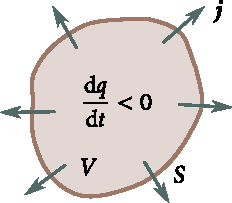
\includegraphics[scale=1]{figures/ch_05/fig_5_1.pdf}
			\caption[]{}
			\label{fig:5_1}
		\end{center}
	\end{minipage}
	\hfill{ }%space{-0.05cm}
	\begin{minipage}[t]{0.48\linewidth}
		\begin{center}
			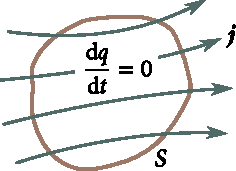
\includegraphics[scale=1]{figures/ch_05/fig_5_2.pdf}
			\caption[]{}
			\label{fig:5_2}
		\end{center}
	\end{minipage}
\vspace{-0.4cm}
\end{figure}

Substituting for $q$ its value $\int_V \rho\,\deriv{V}$, we get the expression
\begin{equation}\label{eq:5_9}
    \oint_S \vec{j} \ccdot \deriv{\vec{S}} = - \diff{}{t} \int_V \rho\, \deriv{V} = - \int_V \diffpartial{\rho}{t}\, \deriv{V}.
\end{equation}

\noindent
We have written the partial derivative of $\rho$ with respect to $t$ inside the integral because the charge density may depend not only on time, but also on the coordinates (the integral $\int_V \rho\,\deriv{V}$ is a function only of time). Let us transform the left-hand side of \eqn{5_9} in accordance with the Ostrogradsky-Gauss theorem. As a result, we get
\begin{equation}\label{eq:5_10}
    \int_V (\divop{\vec{j}})\, \deriv{V} = - \int_V \diffpartial{\rho}{t}\, \deriv{V}.
\end{equation}

\noindent
Equation \eqref{eq:5_10} must be observed upon an arbitrary choice of the volume $V$ over which the integrals are taken. This is possible only if at every point of space the condition is observed that
\begin{equation}\label{eq:5_11}
    \divop{\vec{j}} = - \diffpartial{\rho}{t}.
\end{equation}

\noindent
Equation \eqref{eq:5_11} is known as the \textbf{continuity equation}. It [like \eqn{5_9}] expresses the law of charge conservation. According to \eqn{5_11}, the charge diminishes at points that are sources of the vector $\vec{j}$.

For a steady current, the potential at different points, the charge density, and other quantities are constant. Hence, for a steady current, \eqn{5_11} has the form
\begin{equation}\label{eq:5_12}
    \divop{\vec{j}} = 0.
\end{equation}

\noindent
Thus, for a steady current, the vector $\vec{j}$ has no sources. This signifies that the current lines begin nowhere and terminate nowhere. Hence, the lines of a steady current are always closed. Accordingly, $\oint_S\vec{j}\ccdot\deriv{\vec{S}}$ equals zero. Therefore, for a steady current, the picture similar to that shown in \fig{5_1} has the form shown in \fig{5_2}.

\section{Electromotive Force}\label{sec:5_3}

If an electric field is set up in a conductor and no measures are taken to maintain it, then motion of the current carriers will lead very rapidly to vanishing of the field inside the conductor and stopping of the current. To maintain a current for a sufficiently long time, it is necessary to continuously remove from the end of the conductor with the lower potential (the current carriers are assumed to be positive) the charges carried to it by the current, and continuously supply them to the end with the higher potential (\fig{5_3}). In other words, it is necessary to circulate the charges along a closed path. This agrees with the fact that the lines of a steady current are closed (see the preceding section).

\begin{figure}[t]
	\begin{center}
		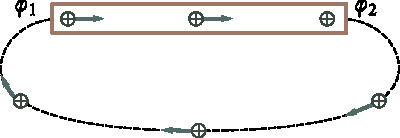
\includegraphics[scale=1]{figures/ch_05/fig_5_3.pdf}
		\caption[]{}
		\label{fig:5_3}
	\end{center}
	\vspace{-0.8cm}
\end{figure}

The circulation of the strength vector of an electrostatic field equals zero. Therefore, in a closed circuit, in addition to sections on which the positive carriers travel in the direction of a decrease in the potential $\varphi$, there must be sections on which the positive charges are carried in the direction of a growth in $\varphi$, \ie, against the forces of the electrostatic field (see the part of the circuit in \fig{5_3} shown by the dash line). Motion of the carriers on these sections is possible only with the aid of forces of a non-electrostatic origin, called \textbf{extraneous forces}. Thus, to maintain a current, extraneous forces are needed that act either over the entire length of the circuit or on separate sections of it. These forces may be due to chemical processes, the diffusion of the current carriers in a non-uniform medium or through the interface between two different substances, to electric (but not electrostatic) fields set up by magnetic fields varying with time (see \sect{9_1}), etc.

Extraneous forces can be characterized by the work they do on charges travelling along a circuit. The quantity equal to the work done by the extraneous forces on a unit positive charge is called the \textbf{electromotive force} (\textbf{e.m.f.}) $\mathcal{E}$ acting in a circuit or on a section of it. Hence, if the work of the extraneous forces on the charge $q$ is $A$, then
\begin{equation}\label{eq:5_13}
    \mathcal{E} = \frac{A}{q}.
\end{equation}

A comparison of \eqns{1_31}{5_13} shows that the dimension of the e.m.f. coincides with that of the potential. Therefore, $\mathcal{E}$ is measured in the same units as $\varphi$.

The extraneous force $\ab{\vec{F}}{extr}$ acting on the charge $q$ can be represented in the form
\begin{equation}\label{eq:5_14}
    \ab{\vec{F}}{extr} = \vec{E}^* q.
\end{equation}

\noindent
The vector quantity $\vec{E}^*$ is called the \textbf{strength of the extraneous force field}. The work (of the extraneous forces on the charge $q$ on circuit section $1$-$2$ is
\begin{equation*}
    A_{12} = \int_1^2 \ab{\vec{F}}{extr}\, \deriv{\vec{l}} = q \int_1^2 \vec{E}^* \ccdot \deriv{\vec{l}}.
\end{equation*}

\noindent
Dividing this work by $q$, we get the e.m.f. acting on the given section:
\begin{equation}\label{eq:5_15}
    \mathcal{E}_{12} = \int_1^2 \vec{E}^* \ccdot \deriv{\vec{l}}.
\end{equation}

\noindent
A similar integral calculated for a closed circuit gives the e.m.f. acting in this circuit:
\begin{equation}\label{eq:5_16}
    \mathcal{E} = \oint \vec{E}^* \ccdot \deriv{\vec{l}}.
\end{equation}

\noindent
Thus, the e.m.f. acting in a closed circuit can be determined as the circulation of the strength vector of the extraneous forces.

In addition to extraneous forces, a charge experiences the forces of an electrostatic field $\vec{F}_E=q\vec{E}$. Hence, the resultant force acting at each point of a circuit on the charge $q$ is
\begin{equation*}
    \vec{F} = \vec{F}_E + \ab{\vec{F}}{extr} = q (\vec{E} + \vec{E}^*).
\end{equation*}

\noindent
The work done by this force on the charge $q$ on circuit section $1$-$2$ is determined by the expression
\begin{equation}\label{eq:5_17}
    A_{12} = q \int_1^2 \vec{E} \ccdot \deriv{\vec{l}} + q \int_1^2 \vec{E}^* \ccdot \deriv{\vec{l}} = q (\varphi_1 - \varphi_2) + q \mathcal{E}_{12}.
\end{equation}

The quantity numerically equal to the work done by the electrostatic and extraneous forces in moving a unit positive charge is defined as the \textbf{voltage drop} or simply the \textbf{voltage} $U$ on the given section of the circuit. According to \eqn{5_17},
\begin{equation}\label{eq:5_18}
    U_{12} = \varphi_1 - \varphi_2 + \mathcal{E}_{12}.
\end{equation}

A section of a circuit on which no extraneous forces act is called \textbf{homogeneous}. A section on which the current carriers experience extraneous forces is called \textbf{inhomogeneous}. For a homogeneous section of a circuit
\begin{equation}\label{eq:5_19}
    U_{12} = \varphi_1 - \varphi_2,
\end{equation}

\noindent
\ie, the voltage coincides with the potential difference across the ends of the section.

\section{Ohm's Law. Resistance of Conductors}\label{sec:5_4}

The German physicist Georg Ohm (1789-1854) experimentally established a law according to which \textit{the current flowing in a homogeneous} (in the meaning that no extraneous forces are present) \textit{metal conductor is proportional to the voltage drop $U$ in the conductor}:
\begin{equation}\label{eq:5_20}
    I = \frac{1}{R} U.
\end{equation}

\noindent
We remind our reader that for a homogeneous conductor the voltage $U$ coincides with the potential difference $\varphi_1-\varphi_2$ [see \eqn{5_18}].

The quantity designated by the symbol $R$ in \eqn{5_20} is called the \textbf{electrical resistance} of a conductor. The unit of resistance is the ohm (\si{\ohm}) equal to the resistance of a conductor in which a current of \SI{1}{\ampere} flows at a voltage of $\SI{1}{\volt}$.

The value of the resistance depends on the shape and dimensions of a conductor and also on the properties of the material it is made of. For a homogeneous cylindrical conductor
\begin{equation}\label{eq:5_21}
    R = \rho \frac{1}{S},
\end{equation}

\noindent
where $l$, is the length of the conductor, $S$ its cross-sectional area, and $\rho$ the coefficient depending on the properties of the material and called the \textbf{resistivity} of the substance.

If $l=1$ and $S=1$, then $R$ numerically equals $\rho$. In the SI, $\rho$ is measured in ohm-metres (\si{\ohm\metre}).

Let us find the relation between the vectors $\vec{j}$ and $\vec{E}$ at the same point of a conductor. In an isotropic conductor, the ordered motion of the current carriers takes place in the direction of the vector $\vec{E}$. Therefore, the directions of the vectors $\vec{j}$ and $\vec{E}$ coincide\footnote{In anisotropic bodies, the directions of the vectors $\vec{j}$ and $\vec{E}$, generally speaking, do not coincide. The relation between $\vec{j}$ and $\vec{E}$ for such bodies is achieved with the aid of the conductance tensor.}. Let us mentally separate an elementary cylindrical volume with generatrices parallel to the vectors $\vec{j}$ and $\vec{E}$ in the vicinity of a certain point (\fig{5_4}).
A current equal to $j\,\deriv{S}$ flows through the cross section of the cylinder. The voltage across the cylinder is $E\,\deriv{l}$, where $E$ is the field-strength at the given point. Finally, the resistance of the cylinder, according to \eqn{5_21}, is $\rho(\diffin{l}{S})$. Using these values in \eqn{5_21}, we arrive at the equation
\begin{equation*}
    j\, \deriv{S} = \frac{1}{\rho} \diff{S}{l} E\, \deriv{l}\quad \text{or}\quad j = \frac{1}{\rho} E.
\end{equation*}

\noindent
Taking advantage of the fact that the vectors $\vec{j}$ and $\vec{E}$ have the same direction, we can write
\begin{equation}\label{eq:5_22}
    \vec{j} = \frac{1}{\rho} \vec{E} = \sigma \vec{E}.
\end{equation}

\noindent
This equation expresses Ohm's law in the differential form.

\begin{figure}[t]
	\begin{center}
		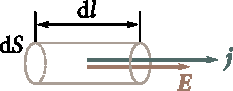
\includegraphics[scale=1]{figures/ch_05/fig_5_4.pdf}
		\caption[]{}
		\label{fig:5_4}
	\end{center}
	\vspace{-0.8cm}
\end{figure}

The quantity $\sigma$ in \eqn{5_22} that is the reciprocal of $\rho$ is called the \textbf{conductivity} of a material. The unit that is the reciprocal of the ohm is called the \textbf{siemens} (\si{\siemens}). The unit of $\sigma$ is accordingly the siemens per metre (\si{\siemens\per\metre}).

Let us assume for simplicity's sake that a conductor contains carriers of only one sign. According to \eqn{5_5}, the current density in this case is
\begin{equation}\label{eq:5_23}
    \vec{j} = e n \vec{u}.
\end{equation}

\noindent
A comparison of this expression with \eqn{5_22} leads us to the conclusion that the velocity of ordered motion of current carriers is proportional to the field strength $\vec{E}$, \ie, to the force imparting ordered motion to the carriers. Proportionality of the velocity to the force applied to a body is observed when apart from the force producing the motion, the body experiences the force of resistance of the medium. This force is due to the interaction of the current carriers with the particles which the substance of the conductor is built of. The presence of the force of resistance to ordered motion of the current carriers results in the electrical resistance of a conductor.

The ability of a substance to conduct an electric current is characterized by its resistivity $\rho$ or conductivity $\sigma$. Their magnitude is determined by the chemical nature of the substance and the surrounding conditions, in particular the ambient temperature.

The resistivity $\rho$ varies directly with the absolute temperature $T$ for most metals at temperatures close to room one:
\begin{equation}\label{eq:5_24}
    \rho \propto T.
\end{equation}

\noindent
Deviations from this proportion are observed at low temperatures (\fig{5_5}). The dependence of $\rho$ on $T$ usually follows curve $1$. The magnitude of the residual resistivity $\ab{\rho}{res}$ depends very greatly on the purity of the material and the presence of residual mechanical stresses in the specimen. This is why $\ab{\rho}{res}$ appreciably diminishes after annealing. The resistivity $\rho$ of a perfectly pure metal with an ideal regular crystal lattice vanishes at absolute zero.

\begin{figure}[t]
	\begin{center}
		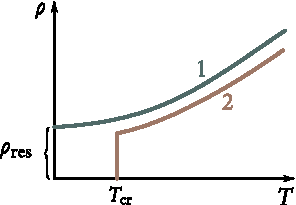
\includegraphics[scale=1]{figures/ch_05/fig_5_5.pdf}
		\caption[]{}
		\label{fig:5_5}
	\end{center}
	\vspace{-0.8cm}
\end{figure}

The resistance of a large group of metals and alloys at a temperature of the order of several kelvins vanishes in a jump (curve $2$ in \fig{5_5}). This phenomenon, called \textbf{superconductivity}, was first discovered in 1911 by the Dutch scientist Heike Kamerlingh Onnes (1853-1926) for mercury. Superconductivity was later discovered in lead, tin, zinc, aluminium, and other metals, as well as in a number of alloys. Every superconductor has its own critical temperature $\ab{T}{cr}$ at which it passes over into a superconducting state. The superconducting state is violated when a magnetic field acts on a superconductor. The magnitude of the critical field $\ab{B}{cr}$ (the symbol $B$ stands for the magnetic induction---see \sect{6_2}) destroying superconductivity equals zero when $T=\ab{T}{cr}$ and grows with lowering of the temperature.

A complete theoretical substantiation of superconductivity was given in 1957 by J. Bardeen, L. Cooper, and J. Schrieffer (see Vol. III, Sec. 8.2).

The temperature dependence of resistance underlies the design of resistance thermometers. Such a thermometer is a metal (usually platinum) wire wound onto a porcelain or mica body. A resistance thermometer graduated according to constant temperature points makes it possible to measure both low and high temperatures with an accuracy of the order of several hundredths of a kelvin. Recent times have seen semiconductor resistance thermometers coming into greater and greater favour.

\section{Ohm's Law for an Inhomogeneous Circuit Section}\label{sec:5_5}

The extraneous forces $e\vec{E}^*$ act on current carriers on an inhomogeneous section of a circuit in addition to the electrostatic forces $e\vec{E}$. Extraneous forces are capable of producing ordered motion of current carriers to the same extent as electrostatic forces are. We found in the preceding section that in a homogeneous conductor, the average velocity of ordered motion of the current carriers is proportional to the electrostatic force $e\vec{E}$. It is quite obvious that, where extraneous forces are exerted on the carriers in addition to the electrostatic forces, the average velocity of ordered motion of the carriers will be proportional to the total force $e\vec{E}+ e\vec{E}^*$. Accordingly, the current density at these points is proportional to the sum of the strengths $\vec{E}+\vec{E}^*$:
\vspace{-12pt}
\begin{equation}\label{eq:5_25}
    \vec{j} = \sigma \parenthesis{\vec{E}+\vec{E}^*}.
\end{equation}

Equation \eqref{eq:5_25} summarizes \eqn{5_22} for an inhomogeneous conductor. It expresses Ohm's law for an inhomogeneous section of a circuit in the differential form.

We can pass over from Ohm's law in the differential form to its integral form. Let us consider an inhomogeneous section of a circuit. Assume that there is a line inside this section (we shall call it the current path) complying with the following conditions: ($1$) in every cross section perpendicular to the path, the quantities $\vec{j}$, $\sigma$, $\vec{E}$, $\vec{E}^*$ have the same values
with sufficient accuracy, and ($2$) the vectors $\vec{j}$, $\vec{E}$, and $\vec{E}^*$ at every point are directed along a tangent to the path. The cross section of the conductor may vary (\fig{5_6}).

\begin{figure}[t]
	\begin{center}
		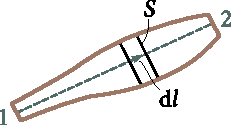
\includegraphics[scale=1]{figures/ch_05/fig_5_6.pdf}
		\caption[]{}
		\label{fig:5_6}
	\end{center}
	\vspace{-0.8cm}
\end{figure}

Let us choose an arbitrary direction of motion along the path. Assume that the chosen \fig{5_6} direction corresponds to motion from end $1$ to end $2$ of the circuit section (direction $1$-$2$). Let us project the vectors in \eqn{5_25} onto the path element $\deriv{\vec{l}}$. The result is
\begin{equation}\label{eq:5_26}
    j_l = \sigma (E_l + E_l^*).
\end{equation}

\noindent
Owing to our assumption, the projection of each of the vectors equals the magnitude of the vector taken with the sign plus or minus depending on the direction of the vector relative to $\deriv{\vec{l}}$. For example, $j_l=j$ if the current flows in direction $1$-$2$, and $j_l=-j$ if it flows in direction $2$-$1$.

Owing to charge conservation, the steady current in each section must be the same. Therefore, the quantity $I=j_lS$ is constant along the path. The current in this case should be treated as an algebraic quantity. We remind our reader that we have chosen direction $1$-$2$ arbitrarily. Hence, if the current flows in the chosen direction, it should be considered positive, and if it flows in the opposite direction (\ie, from end $2$ to end $1$), it should be considered negative.

Let us substitute the ratio $I/S$ for $j_l$ and the resistivity $\rho$ for the conductivity $\sigma$ in \eqn{5_26}. We get
\begin{equation*}
    I \frac{\rho}{S} = E_l + E_l^*.
\end{equation*}

\noindent
Multiplication of the above equation by $\deriv{l}$ and integration along the path yield
\begin{equation*}
    I \int_1^2 \rho\, \frac{\deriv{l}}{S} = \int_1^2 E_l\, \deriv{l} + \int_1^2 E_l^*\, \deriv{l}.
\end{equation*}

\noindent
The quantity $\rho(\deriv{l}/S)$ is the resistance of the path section of length $\deriv{l}$, and the integral of this quantity is the resistance $R$ of the circuit section. The first integral in the right-hand side gives $\varphi_1-\varphi_2$, and the second integral gives the e.m.f. $\mathcal{E}_{12}$ acting on the section. We, thus, arrive at the equation
\begin{equation}\label{eq:5_27}
    I R = \varphi_1 - \varphi_2 + \mathcal{E}_{12}.
\end{equation}

The e.m.f. $\mathcal{E}_{12}$, like the current $I$, is an algebraic quantity. When the e.m.f. facilitates the motion of the positive current carriers in the selected direction (in direction $1$-$2$), we have $\mathcal{E}_{12}>0$. If the e.m.f. prevents the motion of the positive carriers in the given direction, $\mathcal{E}_{12}<0$.

Let us write \eqn{5_27} in the form
\begin{equation}\label{eq:5_28}
    I= \frac{\varphi_1 - \varphi_2 + \mathcal{E}_{12}}{R}.
\end{equation}

\noindent
This equation expresses Ohm's law for an inhomogeneous circuit section. Assuming that $\varphi_1=\varphi_2$, we get the equation of Ohm's law for a closed circuit:
\begin{equation}\label{eq:5_29}
    I= \frac{\mathcal{E}}{R}.
\end{equation}

\noindent
Here, $\mathcal{E}$ is the e.m.f. acting in the circuit, and $R$ is the total resistance of the entire circuit.

\section{Multiloop Circuits. Kirchhoff's Rules}\label{sec:5_6}

The calculation of multiloop circuits or networks is considerably simplified if we use two rules formulated by the German physicist Gustav Kirchhoff (1824-1887). The first of them relates to the junctions of a circuit. A \textbf{junction} is defined as a point where three or more conductors meet (\fig{5_7}). A current flowing toward a junction is considered to have one sign (plus or minus), and a current flowing out of a junction is considered to have the opposite sign (minus or plus).

% \begin{figure}[t]
% 	\begin{center}
% 		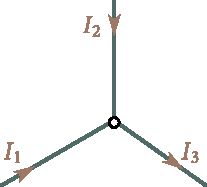
\includegraphics[scale=1]{figures/ch_05/fig_5_7.pdf}
% 		\caption[]{}
% 		\label{fig:5_7}
% 	\end{center}
% 	\vspace{-0.8cm}
% \end{figure}

\begin{figure}[t]
	\begin{minipage}[t]{0.38\linewidth}
		\begin{center}
			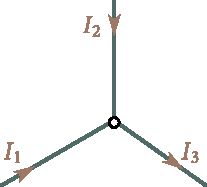
\includegraphics[scale=1]{figures/ch_05/fig_5_7.pdf}
			\caption[]{}
			\label{fig:5_7}
		\end{center}
	\end{minipage}
	\hfill{ }%space{-0.05cm}
	\begin{minipage}[t]{0.58\linewidth}
		\begin{center}
			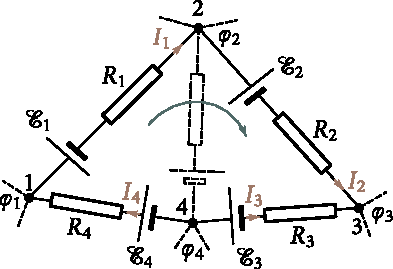
\includegraphics[scale=1]{figures/ch_05/fig_5_8.pdf}
			\caption[]{}
			\label{fig:5_8}
		\end{center}
	\end{minipage}
\vspace{-0.4cm}
\end{figure}

Kirchhoff's first rule, also called the \textbf{junction rule}, states that \textit{the algebraic sum of all the currents coming into a junction must be zero}:
\begin{equation}\label{eq:5_30}
    \sum_k I_k = 0.
\end{equation}

\noindent
This rule follows from the continuity equation, \ie, in the long run from the law of charge conservation. For a steady current, $\divop{\vec{j}}$ equals zero everywhere [see \eqn{5_21}]. Hence, the flux of the vector $\vec{j}$, \ie, the algebraic sum of the currents flowing through an imaginary closed surface surrounding a junction, must be zero.

Equation \eqref{eq:5_30} can be written for each of the $N$ junctions of circuit. Only $N-1$ equations will be independent, however, whereas the $N$-th one will be a corollary of them.

The second rule relates to any closed loop separated from a multiloop circuit (see, for example, loop $1$-$2$-$3$-$4$-$1$ in \fig{5_8}). Let us choose a direction of circumvention (for example, clockwise as in the figure) and apply Ohm's law to each unbranched loop section:
\begin{align*}
    I_1 R_1 &= \varphi_1 - \varphi_2 + \mathcal{E}_1\\
    I_2 R_2 &= \varphi_2 - \varphi_3 + \mathcal{E}_2\\
    I_3 R_3 &= \varphi_3 - \varphi_4 + \mathcal{E}_3\\
    I_4 R_4 &= \varphi_4 - \varphi_1 + \mathcal{E}_4.
\end{align*}

\noindent
When these expressions are summated, the potentials can be cancelled, and we get the equation
\begin{equation}\label{eq:5_31}
    \sum_k I_k R_k = \sum_k \mathcal{E}_k,
\end{equation}

\noindent
that expresses \textbf{Kirchhoff's second rule}, also called the \textbf{loop rule}.

% \begin{figure}[t]
% 	\begin{center}
% 		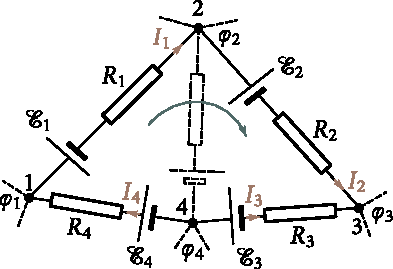
\includegraphics[scale=1]{figures/ch_05/fig_5_8.pdf}
% 		\caption[]{}
% 		\label{fig:5_8}
% 	\end{center}
% 	\vspace{-0.8cm}
% \end{figure}

Equation \eqref{eq:5_31} can be written for all the closed loops that can be separated mentally in a given multiloop circuit. Only the equations for the loops that cannot be obtained by the superposition of
other loops on one another will be independent, however. For example, for the circuit depicted in \fig{5_9}, we can write three equations:
\begin{enumerate}[(1)]
    \item for loop $1$-$2$-$3$-$6$-$1$,
    \item for loop $3$-$4$-$5$-$6$-$3$, and
    \item for loop $1$-$2$-$3$-$4$-$5$-$6$-$1$.
\end{enumerate}

The last loop is obtained by superposition of the first two. The equations will, therefore, not be independent. We can take any two equations of the three as independent ones.

In writing the equations of the loop rule, we must appoint the signs of the currents and e.m.f.'s in accordance with the chosen direction of circumvention. For example, the current $I_1$ in \fig{5_9} must be considered negative because it flows oppositely to the chosen direction of circumvention. The e.m.f. must also be considered negative because it acts in the direction opposite to that of circumvention, and so on.

We may choose the direction of circumvention in each loop absolutely arbitrarily and independently of the choice of the directions in the other loops. It may happen, here, that the same current or the same e.m.f. may be included in different equations with opposite signs (this happens with the current $I_2$ in \fig{5_9} for the indicated directions of circumvention in the loops). This is of no significance, however, because a change in the direction around a loop results only in a reversal of all the signs in \eqn{5_31}.

\begin{figure}[t]
	\begin{center}
		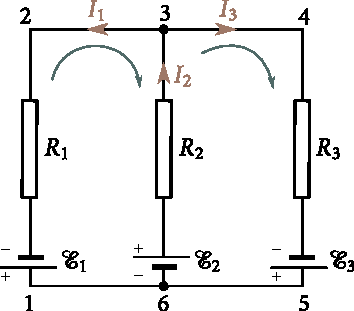
\includegraphics[scale=1]{figures/ch_05/fig_5_9.pdf}
		\caption[]{}
		\label{fig:5_9}
	\end{center}
	\vspace{-0.8cm}
\end{figure}

In compiling the equations, remember that the same current flows in any cross section of an unbranched part of a circuit. For example, the same current $I_2$ flows from junction $6$ to the current source $\mathcal{E}_2$ as from the source $\mathcal{E}_2$ to junction $3$.

The number of independent equations compiled in accordance with the junction and loop rules equals the number of different currents flowing in a multiloop circuit. Therefore, if we know the e.m.f.'s and resistances for all the unbranched sections, we can calculate all the currents. We can also solve other problems, for instance find the e.m.f.'s that must be connected in each of the sections of a circuit to obtain the required currents with the given resistances.

\section{Power of a Current}\label{sec:5_7}

Let us consider an arbitrary section of a steady current circuit across whose ends the voltage $U$ is applied. The charge $q=It$ will flow during the time $t$ through every cross section of the conductor. This is equivalent to the fact that the charge $It$ is carried during the time $t$ from one end of the conductor to the other. The forces of the electrostatic field and the extraneous forces acting on the given section do the work
\begin{equation}\label{eq:5_32}
    A = U q = U I t
\end{equation}

\noindent
[we remind our reader that the voltage $U$ is determined as the work done by the electrostatic and extraneous forces in moving a unit positive charge; see \eqn{5_18}].

Dividing the work $A$ by the time $t$ during which it is done, we get the power developed by the current on the circuit section being considered:
\begin{equation}\label{eq:5_33}
    P = U I = (\varphi_1 - \varphi_2) I + \mathcal{E}_{12} + I.
\end{equation}

\noindent
This power may be spent for the work done by the circuit section being considered on external bodies (for this purpose the section must move in space), for the proceeding of chemical reactions, and, finally, for heating the given circuit section.

The ratio of the power $\Delta{P}$ developed by a current in the volume $\Delta{V}$ of a conductor to the magnitude of this volume is called the \textbf{unit power of the current} $\ab{P}{u}$, corresponding to the given point of the conductor. By definition, the unit power is
\begin{equation}\label{eq:5_34}
    \ab{P}{u} = \frac{\Delta{P}}{\Delta{V}}.
\end{equation}

\noindent
Speaking conditionally, the unit power is the power developed in unit volume of a conductor.

An expression for the unit power can be obtained proceeding from the following considerations. The force $e(\vec{E}+\vec{E}^*)$ develops a power of
\begin{equation*}
    P' = e (\vec{E} + \vec{E}^*) (\vec{v} + \vec{u})
\end{equation*}

\noindent
upon the motion of a current carrier. Let us average this expression for the carriers confined in the volume $\Delta{V}$ within which $\vec{E}$ and $\vec{E}^*$ may be considered constant. The result is
\begin{equation*}
    \average{P'} = e (\vec{E} + \vec{E}^*) \average{\vec{v} + \vec{u}} = e (\vec{E} + \vec{E}^*) \average{\vec{v}} + e (\vec{E} + \vec{E}^*) \average{\vec{u}} = e (\vec{E} + \vec{E}^*) \average{\vec{u}}
\end{equation*}

\noindent
(remember that $\average{\vec{v}}=0$).

We can find the power $\Delta{P}$ developed in the volume $\Delta{V}$ by multiplying $\average{P'}$ by the number of current carriers in this volume, \ie, by $n\Delta{V}$ ($n$ is the number of carriers in unit volume). Thus,
\begin{equation*}
    \Delta{P} = \average{P'} n \Delta{V} = e (\vec{E} + \vec{E}^*) \ccdot \average{\vec{u}} n \Delta{V} = \vec{j} \ccdot (\vec{E} + \vec{E}^*) \Delta{V}
\end{equation*}

\noindent
[see \eqn{5_23}]. Hence,
\begin{equation}\label{eq:5_35}
    \ab{P}{u} = \vec{j} \ccdot (\vec{E} + \vec{E}^*)
\end{equation}

\noindent
This expression is a differential form of the integral equation \eqref{eq:5_33}.

\section{The Joule-Lenz Law}\label{sec:5_8}

When a conductor is stationary and no chemical transformations occur in it, the work of a current given by \eqn{5_32} goes to increase the internal energy of the conductor, and as a result the latter gets heated. It is customary to say that when a current flows in a conductor, the heat
\begin{equation*}
    Q = U I t
\end{equation*}

\noindent
is liberated. Substituting $RI$ for $U$ in accordance with Ohm's law, we get the formula
\vspace{-12pt}
\begin{equation}\label{eq:5_36}
    Q = R I^2 t.
\end{equation}

Equation \eqref{eq:5_36} was established experimentally by the British physicist James Joule (1818-1889) and independently of him by the Russian physicist Emil Lenz (1804-1865), and is called the \textbf{Joule-Lenz law}.

If the current varies with time, then the amount of heat liberated during the time $t$ is calculated by the equation
\begin{equation}\label{eq:5_37}
    Q = \int_0^t R I^2\, \deriv{t}.
\end{equation}

We can pass over from \eqn{5_36} determining the heat liberated in an entire conductor to an expression characterizing the liberation of heat at different spots of the conductor. Let us separate in a conductor, in the same way as we did in deriving \eqn{5_22}, an elementary volume in the form of a cylinder (see \fig{5_4}). According to the Joule-Lenz law, the following amount of heat will be liberated in this volume during the time $\deriv{t}$:
\begin{equation}\label{eq:5_38}
    \deriv{Q} = R I^2\, \deriv{t} = \frac{\rho\, \deriv{l}}{\deriv{S}} (j\, \deriv{S})^2\, \deriv{t} = \rho j^2\, \deriv{V}\, \deriv{t}
\end{equation}

\noindent
($\deriv{V}=\deriv{S}\, \deriv{l}$ is the magnitude of the elementary volume).

Dividing \eqn{5_38} by $\deriv{V}$ and $\deriv{t}$, we shall find the amount of heat liberated in unit volume per unit time:
\begin{equation}\label{eq:5_39}
    \ab{Q}{u} = \rho j^2.
\end{equation}

\noindent
By analogy with the name of quantity \eqn{5_34}, the quantity $\ab{Q}{u}$ can be called the \textbf{unit thermal power of a current}.

Equation \eqref{eq:5_39} is a differential form of the Joule-Lenz law. It can be obtained from \eqn{5_35}. Substituting $\vec{j}/\sigma= \rho\vec{j}$ for $\vec{E}+\vec{E}^*$ in \eqn{5_35} [see \eqn{5_25}], we arrive at the expression
\begin{equation*}
    \ab{P}{u} = \rho \vec{j}^2,
\end{equation*}

\noindent
that coincides with \eqn{5_39}.

It must be noted that Joule and Lenz established their law for a homogeneous circuit section. As follows from what has been said in the present section, however, \eqns{5_36}{5_39} also hold for an inhomogeneous section provided that the extraneous forces acting in it have a non-chemical origin.
